% ============================================================================
% report/methodology.tex — phần "Phương pháp" (fragment, KHÔNG có preamble).
% Dùng qua \input{}; tương thích với pdfLaTeX + inputenc/vietnam.
% Preamble cần: amsmath, booktabs, tabularx, array, graphicx, xcolor, tikz.
% Main có thể dùng BibTeX; mọi trích dẫn bên dưới là \cite{} chuẩn.
% Nội dung chỉ dùng ví dụ schematic; không chép câu thật từ corpus hạn chế.
% ============================================================================

\usetikzlibrary{arrows.meta,positioning,calc,shapes.geometric}

\section{Phương pháp}

Phần này mô tả ba hệ thống dịch Việt--Hán văn được xây dựng trên ngữ liệu
\emph{Đại Việt sử ký toàn thư}: \texttt{E1}, một Transformer huấn luyện từ
đầu bằng Fairseq; \texttt{E2}, mô hình Qwen3-8B được thích nghi bằng QLoRA;
và \texttt{E3-custom}, biến thể của E1 có thêm gợi ý Hán tự được truy hồi ở
phía nguồn. Đây là một \emph{so sánh cấp hệ thống}: ba hệ thống dùng cùng các
cặp câu, cùng định danh mẫu và cùng đường chấm điểm, nhưng khác nhau về biểu
diễn đầu vào, năng lực mô hình, hàm mục tiêu, cách chọn checkpoint và cấu hình
giải mã.

Vì vậy, chênh lệch E1--E2 không thể được quy hoàn toàn cho pretraining, cũng
như chênh lệch E1--E3-custom không phải một ablation sạch của riêng retrieval.
Những yếu tố được kiểm soát và không được kiểm soát được công khai trong
Bảng~\ref{tab:comparison-scope}; phần kết quả nhờ đó có thể diễn giải sức mạnh
của \emph{toàn bộ recipe} mà không gán quan hệ nhân quả vượt quá thiết kế.

\subsection{Thiết kế so sánh và các bất biến dùng chung}

\begin{table}[tbp]
  \centering
  \small
  \renewcommand{\arraystretch}{1.18}
  \caption{Phạm vi kiểm soát của phép so sánh ba hệ thống.}
  \label{tab:comparison-scope}
  \begin{tabularx}{\textwidth}{@{}>{\bfseries}p{3.0cm}XX@{}}
    \toprule
    Trục so sánh & Được giữ chung & Khác giữa các hệ thống \\
    \midrule
    Dữ liệu
      & Cùng split, thứ tự hàng và \texttt{sample\_id}; không dùng target
        validation/test để huấn luyện
      & E3-custom thêm gợi ý vào nguồn; E2 dùng target bỏ khoảng trắng \\
    Tiền xử lý
      & Cùng \texttt{read\_split}, NFC và kiểm tra số dòng
      & Fairseq binarization so với tokenizer/chat template của Qwen3 \\
    Mô hình và mục tiêu
      & Cùng hướng Việt $\rightarrow$ Hán văn
      & From-scratch seq2seq, QLoRA causal LM, seq2seq có augmented source \\
    Lựa chọn mô hình
      & Chỉ dùng validation trước khi mở test
      & E1/E3 chọn bằng BLEU; E2 chọn bằng \texttt{eval\_loss} \\
    Giải mã
      & Không sampling; cấu hình được ghi vào artifact
      & Beam 7 cho E1/E3, beam 4 cho E2; giới hạn độ dài khác nhau \\
    Đánh giá
      & Cùng canonical form, metrics, 510 mẫu và paired bootstrap
      & Không có khác biệt sau trường \texttt{prediction\_scored} \\
    \bottomrule
  \end{tabularx}
\end{table}

Phát biểu chính xác về kiến trúc là \emph{một đầu đọc và một bộ chấm dùng chung},
không phải \emph{chỉ một bước khác nhau}. Hình~\ref{fig:pipeline} thể hiện phần đầu
và cuối dùng chung, cùng ba recipe không đồng nhất ở giữa.

\begin{figure}[tbp]
  \centering
  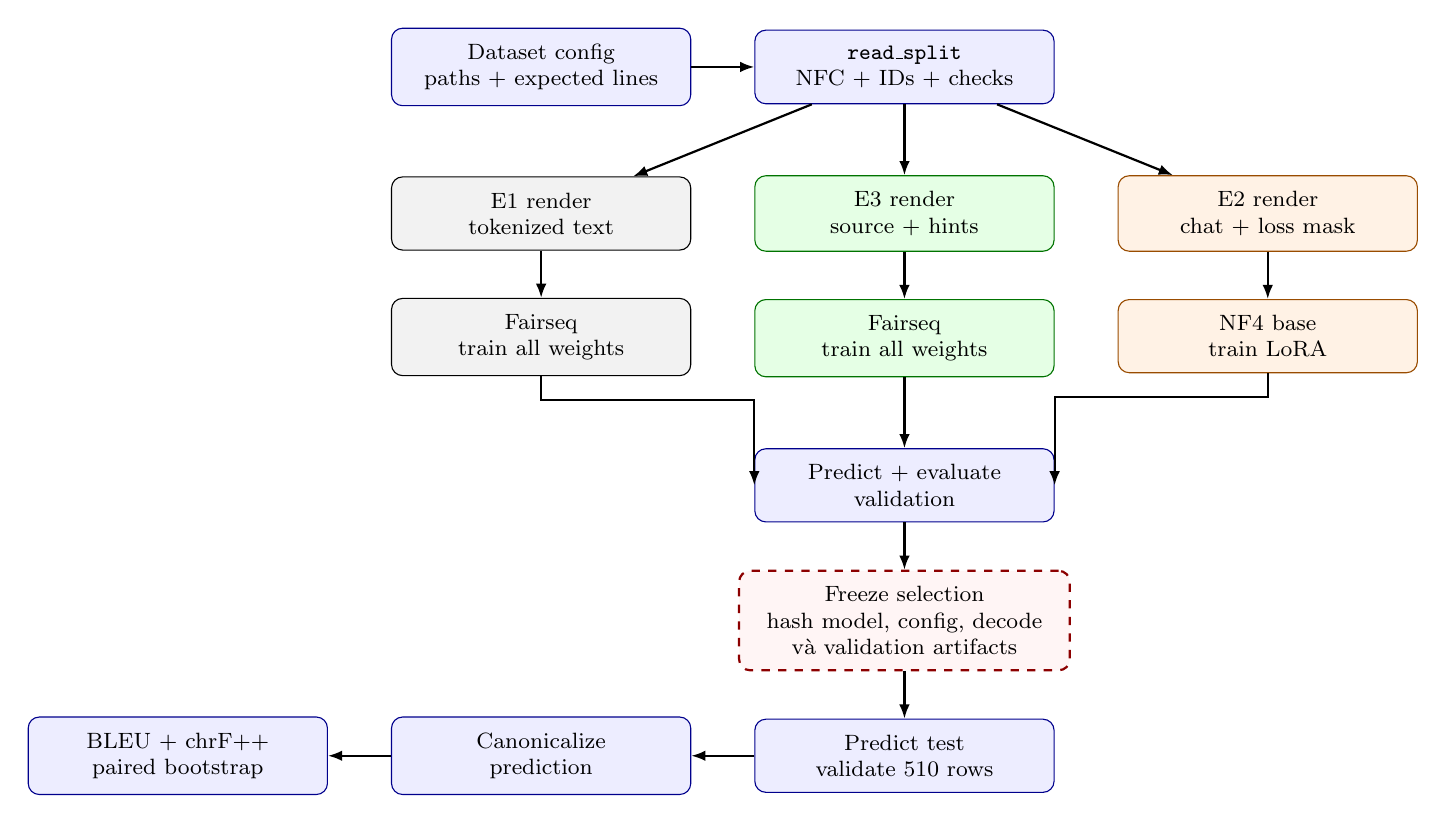
\begin{tikzpicture}[
      font=\footnotesize,node distance=6mm and 8mm,
      box/.style={draw,rounded corners,align=center,minimum height=9mm,
                  text width=34mm,inner sep=2mm},
      shared/.style={box,fill=blue!7,draw=blue!55!black},
      eone/.style={box,fill=gray!10},
      etwo/.style={box,fill=orange!10,draw=orange!60!black},
      ethree/.style={box,fill=green!10,draw=green!45!black},
      gate/.style={box,dashed,thick,text width=38mm,fill=red!4,
                   draw=red!55!black},
      arr/.style={-{Latex[length=1.8mm]},thick}]
    \node[shared] (cfg) {Dataset config\\paths + expected lines};
    \node[shared,right=of cfg] (read) {\texttt{read\_split}\\NFC + IDs + checks};
    \node[ethree,below=9mm of read] (e3r) {E3 render\\source + hints};
    \node[eone,left=of e3r] (e1r) {E1 render\\tokenized text};
    \node[etwo,right=of e3r] (e2r) {E2 render\\chat + loss mask};
    \node[eone,below=of e1r] (e1t) {Fairseq\\train all weights};
    \node[ethree,below=of e3r] (e3t) {Fairseq\\train all weights};
    \node[etwo,below=of e2r] (e2t) {NF4 base\\train LoRA};
    \node[shared,below=9mm of e3t] (val) {Predict + evaluate\\validation};
    \node[gate,below=of val] (freeze) {Freeze selection\\hash model, config, decode\\và validation artifacts};
    \node[shared,below=of freeze] (test) {Predict test\\validate 510 rows};
    \node[shared,left=of test] (score) {Canonicalize\\prediction};
    \node[shared,left=of score] (eval) {BLEU + chrF++\\paired bootstrap};
    \draw[arr] (cfg)--(read);
    \draw[arr] (read)--(e1r); \draw[arr] (read)--(e3r); \draw[arr] (read)--(e2r);
    \draw[arr] (e1r)--(e1t); \draw[arr] (e3r)--(e3t); \draw[arr] (e2r)--(e2t);
    \draw[arr] (e1t.south)--++(0,-3mm)-|(val.west);
    \draw[arr] (e3t)--(val);
    \draw[arr] (e2t.south)--++(0,-3mm)-|(val.east);
    \draw[arr] (val)--(freeze); \draw[arr] (freeze)--(test);
    \draw[arr] (test)--(score); \draw[arr] (score)--(eval);
  \end{tikzpicture}
  \caption{Pipeline cấp hệ thống. Màu xanh lam biểu thị code dùng chung; ba
  màu ở giữa là các recipe; khung nét đứt là cổng khoá tập test.}
  \label{fig:pipeline}
\end{figure}

\subsection{Hợp đồng dữ liệu và biểu diễn văn bản}

\subsubsection{Một đầu đọc duy nhất}

Tất cả đường dẫn corpus nằm trong \texttt{configs/dataset.yaml}. Mỗi split
khai báo hai file song song, nhãn chất lượng và \texttt{expected\_lines}:
19.218 cặp silver, self-aligned cho train; 510 cặp gold, manually aligned cho
validation; và 510 cặp gold cho test. \texttt{read\_split} là đường duy nhất
đưa các file này vào pipeline. Hàm kiểm tra hai vế có cùng số dòng, đối chiếu
số dòng với cấu hình, gán ID ổn định theo thứ tự gốc và chuẩn hoá Unicode NFC
cùng khoảng trắng.

Pipeline không lowercase, không lọc độ dài, không sửa ký tự lỗi và không
deduplicate. Audit tìm thấy 1.596 cặp lặp, 44 nguồn ứng với nhiều target và
sáu hàng train-target chứa U+FFFD. Giữ nguyên giúp bảo toàn corpus được cung
cấp và khả năng đối chiếu; đổi lại, duplicate làm thay đổi trọng số thực
nghiệm và ánh xạ một-nhiều đặt ra giới hạn cho exact matching. NFC là ngoại lệ
cần thiết vì cùng một dấu tiếng Việt có thể có nhiều chuỗi codepoint.

\subsubsection{Ba dạng target cho ba mục đích}

\begin{table}[tbp]
  \centering
  \small
  \renewcommand{\arraystretch}{1.18}
  \caption{Ba biểu diễn của cùng một target; ví dụ hoàn toàn schematic.}
  \label{tab:target-forms}
  \begin{tabularx}{\textwidth}{@{}>{\ttfamily}p{3.3cm}p{4.2cm}X@{}}
    \toprule
    \normalfont\textbf{Trường} & \textbf{Dạng schematic} & \textbf{Vai trò} \\
    \midrule
    reference\_\allowbreak tokenized & \texttt{$c_1$ $c_2$ $c_3$ $\ldots$}
      & Dạng corpus sau NFC; target huấn luyện E1/E3-custom \\
    reference & \texttt{$c_1c_2c_3\ldots$}
      & Bỏ khoảng trắng; target tự nhiên cho E2 và dạng dễ đọc \\
    reference\_scored & \texttt{$c_1$ $c_2$ $c_3$ $\ldots$}
      & Một codepoint trên một token; đầu vào duy nhất của bộ chấm \\
    \bottomrule
  \end{tabularx}
\end{table}

\texttt{score\_form\_chinese} bỏ toàn bộ khoảng trắng rồi tách lại theo
codepoint. Thuộc tính mỗi token Hán là một codepoint đã được kiểm tra trên toàn
bộ 20.238 hàng, nên phép biến đổi không làm thay reference mà chỉ ép output
của các backend về cùng quy ước.

\begin{figure}[tbp]
  \centering
  \begin{tikzpicture}[
      font=\footnotesize,node distance=7mm and 8mm,
      box/.style={draw,rounded corners,align=center,text width=39mm,
                  minimum height=12mm,inner sep=2mm},
      outputbox/.style={draw,rounded corners,align=center,text width=38mm,
                       minimum height=10mm,fill=blue!7},
      arr/.style={-{Latex[length=1.8mm]},thick}]
    \node[box] (row) {\textbf{ParallelRow}\\
      ID: \texttt{test-000042}\\source: $v_1\ v_2\ldots v_n$\\
      target: $c_1\ c_2\ldots c_m$};
    \node[box,below=9mm of row] (e3) {\textbf{E3-custom}\\source + sentinel\\$+h_1\ldots h_k$};
    \node[box,left=of e3] (e1) {\textbf{E1}\\source giữ nguyên\\target cách ký tự};
    \node[box,right=of e3] (e2) {\textbf{E2}\\system/user chat\\assistant: $c_1c_2\ldots c_m$};
    \node[outputbox,below=9mm of e3] (pred) {Backend-specific prediction};
    \node[outputbox,below=of pred] (canon) {$\hat c_1\ \hat c_2\ldots$\\canonical score form};
    \draw[arr] (row)--(e1); \draw[arr] (row)--(e3); \draw[arr] (row)--(e2);
    \draw[arr] (e1.south)--++(0,-3mm)-|(pred.west);
    \draw[arr] (e3)--(pred);
    \draw[arr] (e2.south)--++(0,-3mm)-|(pred.east);
    \draw[arr] (pred)--(canon);
  \end{tikzpicture}
  \caption{Một hàng schematic qua ba cách render và một scoring form; không
  tiết lộ câu thật trong corpus hạn chế.}
  \label{fig:render-contract}
\end{figure}

\subsection{E1: Transformer huấn luyện từ đầu}

E1 sử dụng Transformer encoder--decoder chuẩn~\cite{vaswani2017attention},
triển khai bằng Fairseq~\cite{ott2019fairseq}. Encoder và decoder cùng có sáu
lớp; mỗi lớp dùng biểu diễn 512 chiều, feed-forward 2.048 chiều, tám attention
heads và dropout 0,1. Embedding đầu vào và projection đầu ra của decoder được
chia sẻ. Mô hình có 67.652.608 tham số và toàn bộ tham số được tối ưu, do đó
E1 đóng vai trò baseline không hưởng tri thức từ pretraining.

Ở phía Việt, đơn vị đầu vào là token đã có trong corpus; ở phía Hán, mỗi ký
tự là một token. Fairseq xây dictionary chỉ từ train với
\texttt{thresholdsrc=thresholdtgt=1}; không học BPE và không pruning token đã
xuất hiện trong train. BPE thường giúp NMT xử lý từ hiếm và open vocabulary
\cite{sennrich2016subword}, nhưng target của bài toán đã được phân rã đến cấp
ký tự. Giữ nguyên representation tránh ghép chuỗi Hán tự thành subword phụ
thuộc corpus nhỏ và bảo tồn mọi ký tự đã thấy trong train. Chi phí là
vocabulary cố định vẫn không sinh được ký tự chỉ có ở held-out splits:
validation có 34 và test có 45 target tokens ngoài dictionary train. Vì không
có ablation BPE, đây là một recipe có lý giải, không phải bằng chứng BPE chắc
chắn kém hơn.

Với target $y_{1:T}$, E1 tối thiểu hoá label-smoothed cross-entropy với
$\varepsilon=0{,}1$:
\begin{equation}
  \mathcal{L}_{\mathrm{E1}}
  = -\sum_{t=1}^{T}\left[(1-\varepsilon)\log p(y_t\mid y_{<t},x)
  + \frac{\varepsilon}{|V|}\sum_{v\in V}\log p(v\mid y_{<t},x)\right].
  \label{eq:e1-loss}
\end{equation}
Adam dùng $\beta=(0{,}9,0{,}998)$, learning rate cực đại
$5\times10^{-4}$ và lịch \texttt{inverse\_sqrt} sau 8.000 warmup updates.
Mỗi GPU nhận tối đa 1.000 tokens; \texttt{update\_freq=4} tạo batch hiệu dụng
xấp xỉ 4.000 tokens. Huấn luyện fp16 trên một GPU, tối đa 50.000 updates hoặc
500 epochs, với patience 20 theo validation BLEU. Giải mã dùng beam 7,
length penalty 1,0 và giới hạn $1{,}2|x|+10$ target tokens. Các giá trị này là
cấu hình cố định trước run, không phải kết quả của hyperparameter sweep.

\subsection{E2: Qwen3-8B thích nghi bằng QLoRA}

E2 bắt đầu từ revision cố định của Qwen3-8B (commit được pin trong config)
\cite{qwen3technicalreport}. Thay vì cập nhật tám tỷ tham số, trọng số nền
được lượng tử hoá NF4 4-bit với double quantization và chỉ các adapter LoRA
được huấn luyện~\cite{hu2021lora,dettmers2023qlora}. Với một phép biến đổi
tuyến tính có trọng số đóng băng $W$, adapter học hai ma trận hạng thấp:
\begin{equation}
  h = Wx + \frac{\alpha}{r}BAx,
  \qquad r=16,\quad \alpha=32.
  \label{eq:lora}
\end{equation}
LoRA được gắn vào mọi linear module, dropout bằng 0 và không học bias. Mô hình
được chuẩn bị bằng \texttt{prepare\_model\_for\_kbit\_training} và gradient
checkpointing; phép tính dùng fp16. Đây là đánh đổi trực tiếp giữa chi phí bộ
nhớ và năng lực thích nghi: base model cung cấp prior đa ngôn ngữ mạnh, nhưng
không được cập nhật đầy đủ và đường huấn luyện phụ thuộc kernel lượng tử.

\begin{figure}[tbp]
  \centering
  \begin{tikzpicture}[
      font=\footnotesize,node distance=7mm,
      block/.style={draw,rounded corners,align=center,minimum height=10mm,
                    text width=29mm},
      frozen/.style={block,fill=gray!14},
      trainable/.style={block,fill=orange!14,draw=orange!65!black},
      data/.style={block,fill=blue!7,draw=blue!55!black},
      arr/.style={-{Latex[length=1.8mm]},thick}]
    \node[data] (prompt) {Chat tokens\\prompt + answer};
    \node[frozen,right=of prompt] (base) {Qwen3-8B\\NF4, frozen $W$};
    \node[trainable,above right=2mm and 8mm of base] (a) {LoRA $A$\\$d\rightarrow r$};
    \node[trainable,below right=2mm and 8mm of base] (b) {LoRA $B$\\$r\rightarrow d$};
    \node[data,right=27mm of base] (sum) {$Wx+\frac{\alpha}{r}BAx$\\causal LM logits};
    \node[trainable,right=of sum] (loss) {Loss chỉ trên\\assistant tokens};
    \draw[arr] (prompt)--(base);
    \draw[arr] (base)--node[above,font=\tiny]{frozen path}(sum);
    \draw[arr,orange!75!black] (base.north)|-(a.west);
    \draw[arr,orange!75!black] (a)--(b);
    \draw[arr,orange!75!black] (b.east)-|(sum.south);
    \draw[arr] (sum)--(loss);
  \end{tikzpicture}
  \caption{Luồng tham số của E2. Màu xám là trọng số nền lượng tử và đóng
  băng; màu cam là đường LoRA duy nhất nhận gradient.}
  \label{fig:qlora-path}
\end{figure}

\subsubsection{Chat template và response-only loss}

Mỗi cặp câu được render thành system turn mô tả nhiệm vụ, user turn chứa câu
nguồn và assistant turn chứa Hán văn liền mạch. Qwen3 thinking mode bị tắt ở
cả train và inference để output không lẫn reasoning. Pipeline render hai lần:
một lần đến đầu assistant turn để lấy prefix, và một lần với target đầy đủ.
Nó kiểm tra encoding đầy đủ thực sự bắt đầu bằng prefix trước khi gán
\texttt{-100} cho toàn bộ prefix labels. Vì thế:
\begin{equation}
  \mathcal{L}_{\mathrm{E2}}
  = -\sum_{t:\,m_t=1}\log p(y_t\mid z_{<t}),\qquad
  m_t = \begin{cases}0,&t\in\text{prompt},\\1,&t\in\text{assistant answer}.
  \end{cases}
  \label{eq:response-loss}
\end{equation}
Mục tiêu này ngăn mô hình tiêu tốn gradient để học nhắc lại chỉ dẫn. Assertion
về prefix biến rủi ro âm thầm của chat-template drift thành lỗi dừng rõ ràng.

\begin{figure}[tbp]
  \centering
  \begin{tikzpicture}[
      font=\footnotesize,
      seg/.style={draw,minimum height=11mm,align=center,inner sep=2mm},
      mask/.style={seg,fill=gray!13},
      learn/.style={seg,fill=orange!14,draw=orange!65!black}]
    \node[mask,text width=29mm] (sys) {system instruction\\labels $=-100$};
    \node[mask,text width=27mm,right=0pt of sys] (usr) {user + source\\labels $=-100$};
    \node[mask,text width=18mm,right=0pt of usr] (ast) {assistant\\prefix};
    \node[learn,text width=28mm,right=0pt of ast] (ans) {target tokens\\cross-entropy};
    \node[below=4mm of usr,align=center,font=\scriptsize] (prefix)
      {prefix encoding phải là tiền tố chính xác của full encoding};
    \draw[-{Latex[length=1.5mm]}] (prefix.west)-|(sys.south);
    \draw[-{Latex[length=1.5mm]}] (prefix.east)-|(ast.south);
  \end{tikzpicture}
  \caption{Response-only masking của E2. Chỉ vùng màu cam đóng góp vào loss.}
  \label{fig:response-mask}
\end{figure}

Sau seeded shuffle, các ví dụ hoàn chỉnh được greedy-pack vào cửa sổ 768
tokens; ví dụ không bị cắt đôi nên ranh giới mask vẫn đúng. 19.218 ví dụ trở
thành 2.903 packed sequences, trong khi ví dụ dài nhất chỉ 481 tokens nên việc
hạ giới hạn từ 1.024 xuống 768 sau memory preflight không truncate target.
Packing giảm padding, nhưng attention không được reset giữa các ví dụ trong
cùng cửa sổ; đây là trade-off của recipe, không phải dữ liệu độc lập tuyệt đối
ở tầng attention.

E2 dùng \texttt{paged\_adamw\_8bit}, learning rate $2\times10^{-4}$ theo
cosine, warmup ratio 0,05, weight decay 0,01 và gradient clipping 1,0. Batch
hiệu dụng là 16 packed windows; ba epochs tương ứng 546 updates. Checkpoint
được đánh giá và lưu mỗi 200 steps, chọn theo \texttt{eval\_loss}. Inference
dùng beam 4, không sampling, và
\begin{equation}
  N_{\max}=\min\left(512,\left\lceil2|x|\right\rceil+32\right).
\end{equation}
Không có ablation cho việc chọn \texttt{eval\_loss} thay BLEU hay cho các
hằng số độ dài; chúng được báo cáo như recipe cố định.

\subsection{E3-custom: truy hồi gợi ý Hán tự ở phía nguồn}

E3-custom giữ nguyên các block \texttt{model}, \texttt{training} và
\texttt{decoding} của E1. Can thiệp được khai báo ở tầng dữ liệu: trước khi
binarization, pipeline nối các ký tự Hán ứng viên vào nguồn Việt. Cơ sở tri
thức \texttt{knowledge.json} có 16.000 entries và bao phủ 5.013 trong số
5.458 ký tự target phân biệt của corpus (91,85\%). Coverage chỉ mô tả khả năng
có entry; nó không đảm bảo candidate đúng được truy hồi hoặc mô hình biết sử
dụng candidate.

Chỉ mục gom các chuỗi tra cứu Việt từ \texttt{pronunciation},
\texttt{nom\_query}, \texttt{lookup\_\allowbreak query} và
\texttt{query\_\allowbreak variants}, sau
casefold và chuẩn hoá khoảng trắng. Với source tokens $x_{1:n}$, retriever dò
mọi vị trí bắt đầu và mọi độ dài form đã biết. Mỗi span khớp tăng $m(c,x)$ cho
các ký tự $c$ mà form đó có thể biểu diễn. Candidate được sắp theo khoá:
\begin{equation}
  \operatorname{rank}(c\mid x)
  = \bigl(-m(c,x),\;-f_{\mathrm{train}}(c),\;\operatorname{Unicode}(c)\bigr),
  \label{eq:retrieval-rank}
\end{equation}
trong đó $f_{\mathrm{train}}$ chỉ được tính từ target train. Thành phần thứ hai
không đọc validation/test, còn Unicode tie-break làm kết quả xác định khi hai
ứng viên bằng điểm.

\begin{figure}[tbp]
  \centering
  \begin{tikzpicture}[
      font=\footnotesize,node distance=7mm,
      box/.style={draw,rounded corners,align=center,text width=28mm,
                  minimum height=11mm,inner sep=2mm},
      data/.style={box,fill=green!9,draw=green!45!black},
      warn/.style={box,fill=red!5,draw=red!55!black},
      arr/.style={-{Latex[length=1.8mm]},thick}]
    \node[data] (kb) {Knowledge entries\\6.389 lookup forms};
    \node[data,right=of kb] (match) {Span matching\\count candidates};
    \node[data,right=of match] (rank) {Rank: match count\\train frequency\\Unicode};
    \node[data,right=of rank] (append) {Append sentinel\\top $k\leq64$ hints};
    \node[warn,below=8mm of match] (length) {Nguồn dài $\times3{,}9$\\batch theo câu $\div4$};
    \node[warn,below=8mm of append] (vocab) {Vocabulary $\times4{,}8$\\params $+10{,}3\%$};
    \draw[arr] (kb)--(match); \draw[arr] (match)--(rank); \draw[arr] (rank)--(append);
    \draw[arr] (append.south)--++(0,-3mm)-|(length.east);
    \draw[arr] (append)--(vocab);
  \end{tikzpicture}
  \caption{Retrieval của E3-custom và các hệ quả ngoài ý định. Chỉ sửa source
  vẫn làm thay đổi kích thước mô hình và động lực tối ưu.}
  \label{fig:knowledge-retrieval}
\end{figure}

Nếu có candidate, source được render thành
\texttt{$x_1\ldots x_n$ \_\_knowledge\_\_ $h_1\ldots h_k$}, với
$k\leq64$ và tiếp tục bị giới hạn để không vượt 256 encoder positions. Con số
64 không có ablation hoặc rationale được lưu; artifact cho thấy 100\% hàng
được augment và trung bình 61,5--62,4 candidates, tức retriever gần chạm trần
ở mọi split. Đây là thiết kế high-recall nhưng ít selective.

Augmentation làm train source tăng từ trung bình 20,92 lên 83,44 tokens trước
EOS. Source dictionary tăng từ 3.616 lên 17.264 types. Do E1 chỉ chia sẻ
decoder input/output embeddings, encoder embedding phải thêm
$13.648\times512=6.987.776$ tham số; tổng mô hình tăng từ 67.652.608 lên
74.640.384 tham số. Cùng giới hạn 1.000 tokens/GPU vì thế chứa ít câu hơn.
E1--E3-custom là phép so sánh hai recipe có chung cấu hình khai báo nhưng
không cùng model size hay realized sentence batch; không nên gọi đây là đo
lường cô lập tác động retrieval.

\paragraph{Ranh giới với E3 chính thức.}
\texttt{e3\_fairseq\_knowledge} trong đặc tả phòng lab yêu cầu integration
\texttt{knowledge\_v2} chưa được cung cấp và backend chủ động dừng. Hệ thống
đã chạy mang ID riêng
\texttt{e3\_custom\_fairseq\_knowledge\_vi\_zh\_v1}; mọi bảng và diễn giải
phải giữ hậu tố \emph{custom}. E4 (Qwen3 cộng cùng retrieval) chỉ được triển
khai và preflight, chưa huấn luyện nên nằm ngoài phương pháp thực nghiệm này.

\subsection{Tổng hợp cấu hình và realized protocol}

Bảng~\ref{tab:configs} so sánh recipe được khai báo. Batch Fairseq là
token-based, còn E2 là packed-window-based, nên không thể đặt chúng trên cùng
một thang số câu mỗi update.

\begin{table}[tbp]
  \centering
  \footnotesize
  \renewcommand{\arraystretch}{1.16}
  \setlength{\tabcolsep}{3.5pt}
  \caption{Cấu hình mô hình, huấn luyện và giải mã.}
  \label{tab:configs}
  \begin{tabularx}{\textwidth}{@{}>{\bfseries}p{2.45cm}XXX@{}}
    \toprule
    Thuộc tính & E1 & E2 & E3-custom \\
    \midrule
    Backbone
      & Transformer 6+6, $d=512$
      & Qwen3-8B NF4 + LoRA $r=16$
      & Giống E1, augmented source \\
    Tham số
      & 67,65M, train toàn bộ
      & 8B frozen + LoRA trainable
      & 74,64M, train toàn bộ \\
    Target train
      & Character-spaced & Hán văn liền mạch & Character-spaced \\
    Objective
      & Label-smoothed CE 0,1 & Response-only causal CE & Giống E1 \\
    Optimizer
      & Adam, $5\times10^{-4}$, inverse-sqrt
      & Paged AdamW 8-bit, $2\times10^{-4}$, cosine
      & Giống E1 \\
    Batch khai báo
      & 1.000 tokens $\times$ accumulation 4
      & 1 window $\times$ accumulation 16
      & Giống E1 \\
    Chọn checkpoint
      & Validation BLEU, patience 20
      & Validation loss, mỗi 200 steps
      & Validation BLEU, patience 20 \\
    Decode
      & Beam 7; $1{,}2|x|+10$
      & Beam 4; $\min(512,\lceil2|x|\rceil+32)$
      & Giống E1 \\
    \bottomrule
  \end{tabularx}
\end{table}

Configured protocol và realized run khác nhau đáng kể
(Bảng~\ref{tab:realized}). Việc báo cả hai ngăn các giới hạn như
\texttt{max\_update} bị hiểu nhầm thành lượng huấn luyện thực tế.

\begin{table}[tbp]
  \centering
  \footnotesize
  \renewcommand{\arraystretch}{1.18}
  \caption{Cấu hình dừng/chọn mô hình so với hành vi thực tế của các run đã
  tạo artifact. Đây là thông tin phương pháp, không phải kết quả dịch.}
  \label{tab:realized}
  \begin{tabularx}{\textwidth}{@{}>{\bfseries}p{2.2cm}XXX@{}}
    \toprule
    & E1 & E2 & E3-custom \\
    \midrule
    Giới hạn
      & 50k updates; 500 epochs; patience 20
      & 3 epochs = 546 steps
      & Như E1 \\
    Thực tế
      & Dừng epoch 171, update 24.791
      & Hoàn tất 546 steps
      & Chạm 50.000 updates ở epoch 87 \\
    Checkpoint chọn
      & Best BLEU ở epoch 151
      & Best loss ở step 400; chỉ hai điểm eval
      & Best BLEU ở epoch 77 \\
    Batch quan sát
      & 132,5 câu/update trung bình
      & 16 packed windows/update
      & 33,3 câu/update trung bình \\
    Caveat chính
      & Checkpoint nối tiếp một lần chạy bị ngắt
      & Freeze record không khớp byte với config hiện tại
      & Không budget-matched với E1 \\
    \bottomrule
  \end{tabularx}
\end{table}

Ba caveat cuối không làm thay đổi prediction hay metric đã lưu, nhưng giới hạn
phát biểu về tái lập và quan hệ nhân quả. E1 có checkpoint kiểm chứng được,
song không tái tạo từ một clean command đơn lẻ vì đã resume ở epoch 5/update
579. Với E2, training config và decoding block còn trong manifest/prediction
rows, nhưng trạng thái \texttt{prompt} và \texttt{model.*} tại đúng thời điểm
test generation không thể chứng minh từ freeze record hiện tại. Các chi tiết
này cần được nhắc lại ở phần Hạn chế thay vì bị che bởi một tuyên bố
reproducible chung.

\subsection{Lựa chọn trên validation và khoá tập test}

Mỗi hệ thống lần lượt huấn luyện, dự đoán và chấm validation, đóng băng lựa
chọn, rồi mới dự đoán test. \texttt{freeze-selection} ghi hash của config,
checkpoint/adapter, decoding block, validation predictions và validation
metrics. Trước mỗi test decode, \texttt{ensure\_selection\_frozen} tính lại
các giá trị này. Một thay đổi hậu nghiệm vào model hoặc beam settings làm
pipeline dừng thay vì sinh một test score mới.

\begin{figure}[tbp]
  \centering
  \begin{tikzpicture}[
      font=\footnotesize,node distance=7mm,
      flowstep/.style={draw,rounded corners,align=center,minimum height=9mm,
                       text width=28mm,fill=blue!7},
      gate/.style={draw,diamond,aspect=2.2,align=center,inner sep=1.5mm,
                   fill=red!5,draw=red!55!black},
      arr/.style={-{Latex[length=1.8mm]},thick}]
    \node[flowstep] (train) {Train};
    \node[flowstep,right=of train] (valp) {Predict + score\\validation};
    \node[flowstep,right=of valp] (select) {Select\\checkpoint};
    \node[gate,below=8mm of select] (freeze) {hash\\match?};
    \node[flowstep,below left=9mm and 8mm of freeze] (test) {Predict\\test};
    \node[flowstep,below=of test] (metric) {Canonical score\\+ bootstrap};
    \node[below right=9mm and 8mm of freeze,align=center,text width=38mm] (stop)
      {Dừng nếu config, checkpoint, decode hoặc validation artifact đổi};
    \draw[arr] (train)--(valp); \draw[arr] (valp)--(select);
    \draw[arr] (select)--(freeze);
    \draw[arr] (freeze.south west)--node[left,font=\scriptsize]{yes}(test.north);
    \draw[arr] (test)--(metric);
    \draw[-{Latex[length=1.8mm]},thick,red!65!black]
      (freeze.south east)--node[right,font=\scriptsize]{no}(stop.north);
  \end{tikzpicture}
  \caption{Cổng validation--test biến chính sách không tune trên test thành
  một điều kiện được kiểm tra bằng hash.}
  \label{fig:freeze-gate}
\end{figure}

Cổng này bảo vệ \emph{quy trình} chứ không làm selection criteria giống nhau.
E1/E3 dùng BLEU nội bộ của Fairseq, còn E2 dùng loss và chỉ có hai điểm
evaluation. Phép so sánh cuối phản ánh cả chiến lược chọn checkpoint. Không có
post-hoc thay đổi selection nào để làm chúng đồng nhất sau khi test đã sinh.

\subsection{Chấm điểm và so sánh thống kê}

\subsubsection{Canonical character-level metrics}

Mỗi prediction JSONL phải có đúng 510 hàng theo cùng thứ tự ID, không trùng ID
và chỉ chứa một experiment/split. Trước khi chấm, evaluator tự tính lại
\texttt{score\_form\_\allowbreak chinese(prediction)} và từ chối file nếu giá trị này khác
\texttt{prediction\_scored}. Kiểm tra này ngăn output đã chỉnh tay hoặc
canonicalize bằng code khác đi vào metric.

BLEU được tính bằng SacreBLEU~\cite{papineni2002bleu,post2018sacrebleu}; chrF++
theo Popovi\'c~\cite{popovic2017chrfpp}. Cấu hình chính xác nằm trong
Bảng~\ref{tab:metrics}. Vì upstream đã chèn khoảng trắng giữa mọi codepoint,
\texttt{tok:13a} gần như không còn đơn vị từ để phân đoạn: BLEU trong báo cáo
là character-level BLEU. Tương tự, với \texttt{whitespace=false}, word
bigrams của chrF++ hoạt động trên các đơn vị được cách sẵn, tức trên ký tự.
Các điểm này so sánh hợp lệ giữa ba hệ thống ở đây, nhưng không cùng thang với
word-level BLEU trên target tiếng Anh hoặc tiếng Việt.

\begin{table}[tbp]
  \centering
  \small
  \renewcommand{\arraystretch}{1.18}
  \caption{Cấu hình đánh giá được lưu trong mọi metrics artifact.}
  \label{tab:metrics}
  \begin{tabularx}{\textwidth}{@{}>{\bfseries}p{2.5cm}p{4.7cm}X@{}}
    \toprule
    Thành phần & Thiết lập & Ý nghĩa \\
    \midrule
    SacreBLEU
      & v2.6.0; case mixed; tokenizer 13a; exponential smoothing; effective order off
      & Corpus BLEU 1--4 gram trên chuỗi character-spaced \\
    chrF2++
      & v2.6.0; $n_c=6$; $n_w=2$; $\beta=2$; whitespace off
      & F-score ưu tiên recall, kết hợp character và \emph{word} n-grams \\
    Test unit
      & 510 paired \texttt{sample\_id}s, một reference mỗi mẫu
      & Giữ độ khó câu giống nhau trong mọi system comparison \\
    Bootstrap
      & 1.000 resamples, seed 42, percentile interval 2,5/97,5
      & Ước lượng bất định của chênh lệch corpus metric \\
    \bottomrule
  \end{tabularx}
\end{table}

\subsubsection{Paired bootstrap}

Với hai hệ thống $A,B$ và $N=510$ IDs, mỗi bootstrap replicate lấy $N$ chỉ
số có hoàn lại, rồi tính lại toàn bộ corpus metric trên cùng tập chỉ số cho cả
hai hệ thống~\cite{koehn2004statistical}. Nếu $M$ là BLEU hoặc chrF++, delta
của replicate $b$ là
\begin{equation}
  \Delta^{(b)}=M\!\left(B_{I_b},R_{I_b}\right)
                 -M\!\left(A_{I_b},R_{I_b}\right),
  \qquad b=1,\ldots,1000.
\end{equation}
Khoảng 95\% lấy percentile 2,5 và 97,5 của các $\Delta^{(b)}$. P-value hai
phía dùng tail nhỏ hơn, nhân hai, với hiệu chỉnh $+1$ ở tử và mẫu để tránh
ước lượng bằng không. Pairing loại bỏ biến thiên do hai hệ thống vô tình nhận
hai tập câu khác độ khó; nó không sửa confound về model, training hay
selection đã nêu ở trên.

\subsection{Tổng hợp quyết định, phương án thay thế và chi phí}

Bảng~\ref{tab:decisions} phân biệt ba mức provenance. \emph{Có tài liệu} là lý
do đã có trong đặc tả hoặc tài liệu dự án; \emph{từ code} là lý do có thể suy
ra trực tiếp từ implementation/artifact; \emph{chưa ablate} chỉ là recipe đã
chạy, không có bằng chứng so sánh với phương án khác.

\begin{table}[tbp]
  \centering
  \scriptsize
  \renewcommand{\arraystretch}{1.18}
  \setlength{\tabcolsep}{3pt}
  \caption{Các quyết định phương pháp và giới hạn diễn giải.}
  \label{tab:decisions}
  \begin{tabularx}{\textwidth}{@{}p{2.35cm}p{2.05cm}XXp{1.7cm}@{}}
    \toprule
    \textbf{Quyết định} & \textbf{Thay thế} & \textbf{Lý do}
      & \textbf{Chi phí/giới hạn} & \textbf{Nguồn} \\
    \midrule
    Không BPE; threshold 1
      & BPE/prune vocab
      & Target đã là một ký tự/token; giữ ký tự hiếm trong train
      & Vẫn có held-out OOV; chưa ablate
      & Có tài liệu \\
    Giữ duplicate và U+FFFD
      & Làm sạch corpus
      & Không phỏng đoán ký tự mất; giữ corpus gốc
      & Duplicate reweight; 44 nguồn đa target
      & Có tài liệu \\
    E2 target liền mạch
      & Character-spaced
      & Phù hợp bề mặt pretrained LM đã gặp
      & Cần canonicalization trước scoring
      & Từ code \\
    Response-only loss
      & Loss cả prompt
      & Tối ưu trực tiếp phần dịch
      & Phụ thuộc prefix-mask; có assertion bảo vệ
      & Từ code \\
    E2 packing
      & Một ví dụ/window
      & Giảm padding, vừa ngân sách GPU
      & Không reset attention giữa ví dụ
      & Từ code \\
    Tối đa 64 hints
      & Budget nhỏ/học scorer
      & Không có rationale được lưu
      & Gần bão hoà; source dài $\sim3{,}9\times$
      & Chưa ablate \\
    Rank bằng train frequency
      & Tần suất mọi split
      & Deterministic, không đọc held-out target
      & Frequency không đo đúng nghĩa theo ngữ cảnh
      & Từ code \\
    E2 chọn bằng loss
      & Chọn BLEU
      & Trainer recipe cố định
      & Criteria khác E1/E3; chỉ hai eval points
      & Chưa ablate \\
    Character-level scoring
      & Mỗi backend tự tokenize
      & Đặt mọi output trên cùng bề mặt
      & Không so trực tiếp với word-level BLEU
      & Có tài liệu \\
    Freeze gate trước test
      & Quy ước thủ công
      & Cơ học hoá cam kết không tune trên test
      & Config drift làm generation bị chặn
      & Có tài liệu \\
    \bottomrule
  \end{tabularx}
\end{table}

Tóm lại, độ tin cậy của phép so sánh đến từ ba invariant: cùng các hàng dữ
liệu, test chỉ mở sau khi selection được đóng băng, và mọi prediction được
chấm bằng cùng canonical evaluator. Những invariant này đủ để so sánh hiệu
năng của ba \emph{hệ thống đã triển khai}; chúng không biến khác biệt recipe
thành một thí nghiệm nhân quả. Giữ ranh giới đó là điều kiện để phần Kết quả
và Hạn chế diễn giải chênh lệch một cách trung thực.
